\begin{enumerate}
\item La stratégie d'énumération des couples d'entier peut être visualisée sur un graphique en suivant les diagonales successives comme sur l'image\footnote{Image provenant de Wikipedia, ce fichier est disponible selon les termes de la licence
 Creative Commons.} suivante :
\begin{figure*}[!h]
\begin{center}
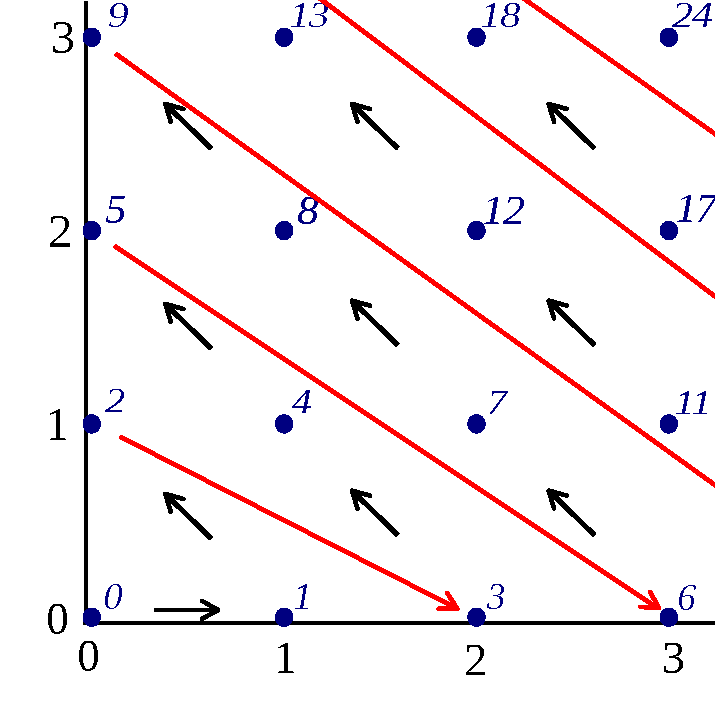
\includegraphics[width=0.6\textwidth]{files/diagcouples.pdf}
\caption{La fonction de couplage de Cantor établit une bijection de $\mathbb{N}*\mathbb{N}$ dans
 $\mathbb{N}$.}
 \end{center}
\end{figure*}

Soit $(x,y) \in \mathbb{N}*\mathbb{N}$ un couple. On trie par ordre lexicographique $(x+y)$. Ainsi on obtient le tableau suivant :

\begin{tabularx}{1.1\textwidth}{| m{1.5cm} | X | X | X | X | X | X | X | X | X | X | X }
\hline
$(x,y)$ & $(0,0)$ & $(1,0)$ & $(0,1)$ & $(2,0)$ & $(1,1)$ & $(0,2)$ & $(3,0)$ & $(2,1)$ & $(1,2)$ & $(0,3)$ & \ldots \\
\hline
$(x+y)$ & 0 & 1 & 1 & 2 & 2 & 2 & 3 & 3 & 3 & 3 & \ldots \\
\hline
$c_2(x+y)$ & 0 & 1 & 2 & 3 & 4 & 5 & 6 & 7 & 8 & 9 & \ldots \\
\hline
\end{tabularx}

\item
\begin{description}
\item[Fonction de codage]
\[ c_2(x,y)= \frac{(x+y)(x+y+1)}{2}+y \]

\item[Fonctions de décodage]
Les fonctions de décodage ne peuvent pas être décrites sous la forme de formules arithmétiques. Elles nécessitent l'algorithme suivant :

\begin{algorithm}[H]
  \caption{CalculXY}
  \Donnees{\\
  $z$; \textit{// Rang du couple (x,y)}
  }
  \Deb{
  $s \leftarrow 0$\;
  $t \leftarrow 0$\;
    \Tq{$s \leqslant z$}{
		$s \leftarrow \frac{t*(t+1)}{2}$\;
		$t \leftarrow t+1$\;
    }
    $t \leftarrow t-2$\;
    $z \leftarrow \frac{t*(t+1)}{2}$\;
    $y \leftarrow z-s$\;
    $x \leftarrow t-y$\;
    \Retour Couple($x$,$y$)\;
  }
\end{algorithm}
\end{description}

\item 
\begin{description}
\item[Codage des triplets] : il peut avoir lieu de manière récursive :
\[ c_3(x,y,z)=c_2(x,c_2(y,z)) \]
\item[Généralisation au codage des k-uplets] : 
\begin{eqnarray*}
& &c_k(x_1,x_2,\ldots,x_k)=c_2(x_1,c_{k-1}(x_2,\ldots,x_k)) \\
\textrm{Avec : } & &c_2(x,y)=\frac{(x+y)(x+y+1)}{2}+y
\end{eqnarray*}



\end{description}

\end{enumerate}